\chapter{บทนำ}
%%%%%%%%%%%%%%%%%%%%%%%%%%%%%%%%%%%%%%%%%%%%%%%%%%%%%%%%%%%%%%%%%%%%%%%%%%%%%%%
\section{ที่มาและความสำคัญ}
บริษัท เพอเซ็ปทรา ดำเนินธุรกิจเกี่ยวกับการให้บริการและคำปรึกษาเกี่ยวกับปัญญาประดิษฐ์ (artificial intelligence)
เนื่องจากปัจจุบันนั้นความสามารถและประสิทธิภาพของปัญญาประดิษฐ์มีความก้าวหน้าขึ้นจนสามารถก้าวข้ามความสามารถของมนุษย์ในงานหลายๆประเภท
ทำให้ลูกค้านั้นมีความต้องการที่จะให้ทางบริษัทสร้างปัญญาประดิษฐ์เพื่อนำไปใช้งานหรือแก้ปัญหาที่ต่างกันออกไป เช่น ใช้ปัญญาประดิษฐ์มาช่วยประมวลผลภาพจากกล้องวงจรปิด เพื่อหาบุคคลที่มีท่าทางน่าสงสัย เป็นต้น
ซึ่งการจะสร้างปัญญาประดิษฐ์ที่เหมาะสมกับการแก้ปัญหาเหล่านั้น จำเป็นต้องมีชุดข้อมูล (dataset) ที่เหมาะสม บางครั้งอาจต้องใช้มนุษย์ในการสร้างขึ้นมาโดยการเก็บข้อมูลวิดีโอ 
และลงมือสร้างชุดข้อมูลจากวิดีโอที่ได้ด้วยตัวเอง ซึ่งหนึ่งในปัจจัยสำคัญในการพัฒนาโมเดลปัญญาประดิษฐ์ให้มีประสิทธิภาพสูงคือจำนวนข้อมูล
ซึ่งหากมีจำนวนวิดีโอเป็นจำนวนมาก การใช้มนุษย์ในการสร้างชุดข้อมูลนั้นอาจจะต้องใช้มนุษย์เป็นจำนวนมาก และใช้เวลานาน 

ทางคณะผู้วิจัยจึงมีความต้องการที่จะออกแบบและพัฒนาระบบต้นแบบของเครื่องมือสำหรับกำกับข้อมูลด้วยปัญญาประดิษฐ์ (A.I.-assisted video labeling tool) สำหรับสร้างชุดข้อมูลจากวิดีโอ 
เพื่อช่วยแบ่งเบาภาระของผู้พัฒนาในการสร้างชุดข้อมูลสำหรับการพัฒนาโมเดลปัญญาประดิษฐ์ในการใช้แก้ปัญหาที่ลูกค้าต้องการ 
โดยโครงการสหกิจนี้เน้นศึกษาเกี่ยวกับการวิเคราะห์และจดจำการกระทำของมนุษย์ภายในสำนักงานจากภาพเคลื่อนไหวเป็นหลัก

%%%%%%%%%%%%%%%%%%%%%%%%%%%%%%%%%%%%%%%%%%%%%%%%%%%%%%%%%%%%%%%%%%%%%%%%%%%%%%%
\section{วัตถุประสงค์}
\begin{enumerate}
	\setlength\itemsep{-0.25em}
	\item เพื่อพัฒนาระบบต้นแบบของเครื่องมือสำหรับกำกับข้อมูลด้วยปัญญาประดิษฐ์ ที่ทำให้มนุษย์กับปัญญาประดิษฐ์ทำงานร่วมกันเพื่อสร้างชุดข้อมูลในการนำมาพัฒนาปัญญาประดิษฐ์อื่นๆที่เหมาะสมกับปัญหาที่ต้องการ
	\item เพื่อออกแบบและสร้างระบบต้นแบบวิเคราะห์วิดีโอที่สามารถตรวจจับมนุษย์และจำแนกการกระทำพื้นฐานของมนุษย์ภายในสำนักงาน ประกอบด้วย ยืน นั่ง เดิน เล่นโทรศัพท์ กินข้าว พูดคุย นอน โดยใช้ปัญญาประดิษฐ์
	\item เพื่อพัฒนาเครื่องมือที่สามารถสร้างชุดข้อมูลสำหรับการจดจำการกระทำของมนุษย์ให้สามารถใช้งานได้ง่าย สะดวกสบายมากขึ้น และมีประสิทธิภาพที่สูงกว่าเครื่องมือตัวอื่นในปัจจุบัน
\end{enumerate}

%%%%%%%%%%%%%%%%%%%%%%%%%%%%%%%%%%%%%%%%%%%%%%%%%%%%%%%%%%%%%%%%%%%%%%%%%%%%%%%

\section{ประโยชน์ที่คาดว่าจะได้รับ}
\begin{enumerate}
	\setlength\itemsep{-0.25em}
	\item เพิ่มความสะดวกในการสร้างชุดข้อมูลสำหรับพัฒนาโมเดลปัญญาประดิษฐ์จากวิดีโอ
	\item ต้นแบบระบบวิเคราะห์วิดีโอที่สามารถจำแนกการกระทำของมนุษย์ภายในสำนักงานได้
\end{enumerate}
\clearpage

%%%%%%%%%%%%%%%%%%%%%%%%%%%%%%%%%%%%%%%%%%%%%%%%%%%%%%%%%%%%%%%%%%%%%%%%%%%%%%%
\section{ขอบเขตการดำเนินงาน}
\begin{enumerate}
	\setlength\itemsep{-0.25em}
	\item สร้างระบบต้นแบบของเครื่องมือสำหรับกำกับข้อมูลด้วยปัญญาประดิษฐ์ โดยระบบจะประกอบไปด้วยสี่ส่วนดังนี้
	\begin{enumerate}
		\setlength\itemsep{-0.25em}
		\item หน้าต่างของแอพพลิเคชั่น (user interface)
		\item ระบบตรวจจับมนุษย์ในภาพ
		\item ระบบทำนายตำแหน่งต่อไปของมนุษย์ในภาพเคลื่อนไหว
		\item ระบบจำแนกการกระทำของมนุษย์ ซึ่งประกอบไปด้วย ยืน นั่ง เดิน เล่นโทรศัพท์ กินข้าว พูดคุย นอน
	\end{enumerate}
	\item ทดสอบโมเดลปัญญาประดิษฐ์สำหรับจำแนกการกระทำของมนุษย์กับชุดข้อมูลที่ได้จากเครื่องมือสำหรับกำกับข้อมูลด้วยปัญญาประดิษฐ์ เพื่อที่จะทดสอบว่าชุดข้อมูลที่ได้สามารถใช้งานจริงได้หรือไม่
	\item พัฒนาโมเดลปัญญาประดิษฐ์สำหรับจำแนกการกระทำของมนุษย์ภายในสำนักงานอย่างน้อย 2 โมเดล
\end{enumerate}

%%%%%%%%%%%%%%%%%%%%%%%%%%%%%%%%%%%%%%%%%%%%%%%%%%%%%%%%%%%%%%%%%%%%%%%%%%%%%%%
\section{ขั้นตอนการดำเนินงาน}
การดำเนินงานวิจัยถูกแบ่งออกเป็นสามส่วน โดยส่วนแรกคือการศึกษาเทคโนโลยีในปัจจุบันเพื่อหาความเป็นไปได้และกำหนดขอบเขตของงาน 
ส่วนที่สองคือเครื่องมือสำหรับกำกับข้อมูลด้วยปัญญาประดิษฐ์ เป็นส่วนที่ออกแบบและพัฒนาเครื่องมือสำหรับช่วยผู้พัฒนาในการสร้างชุดข้อมูล 
และส่วนที่สุดท้ายคือการนำชุดข้อมูลที่ได้จากการใช้เครื่องมือสำหรับกำกับข้อมูลด้วยปัญญาประดิษฐ์ไปพัฒนาโมเดลปัญญาประดิษฐ์สำหรับการจำแนกการกระทำของมนุษย์ภายในสำนักงาน
\subsection*{ศึกษาค้นคว้าเอกสารและงานวิจัยที่เกี่ยวข้อง}
\begin{enumerate}\setlength\itemsep{-0.25em}
	\item ศึกษาเกี่ยวกับการวิเคราะห์วิดิโอ (video analytics)
	\item ศึกษาเกี่ยวกับชุดข้อมูลสำหรับการวิเคราะห์ผลวิดีโอ
	\item ศึกษาเกี่ยวกับโมเดลปัญญาประดิษฐ์ที่ใช้ในการวิเคราะห์วิดีโอ
	\item ศึกษาเครื่องมือที่ใช้ในการช่วยสร้างชุดข้อมูลจากวิดีโอ
\end{enumerate}
\subsection*{เครื่องมือสำหรับกำกับข้อมูลด้วยปัญญาประดิษฐ์}
\begin{enumerate}\setlength\itemsep{-0.25em}
	\item ออกแบบและสร้างหน้าต่างแอพพลิเคชั่นของเครื่องมือสำหรับกำกับข้อมูลด้วยปัญญาประดิษฐ์
	\item ออกแบบและสร้างระบบของเครื่องมือสำหรับกำกับข้อมูลด้วยปัญญาประดิษฐ์
	\item ทดสอบและปรับปรุงการทำงานของเครื่องมือสำหรับกำกับข้อมูลด้วยปัญญาประดิษฐ์
\end{enumerate}
\subsection*{โมเดลปัญญาประดิษฐ์สำหรับการจำแนกการกระทำของมนุษย์ภายในสำนักงาน}
\begin{enumerate}\setlength\itemsep{-0.25em}
	\item สร้างชุดข้อมูลสำหรับสร้างโมเดลปัญญาประดิษฐ์จากเครื่องมือสำหรับกำกับข้อมูลด้วยปัญญาประดิษฐ์
	\item สร้างโมเดลปัญญาประดิษฐ์สำหรับการจำแนกการกระทำของมนุษย์ภายในสำนักงาน
	\item ทดสอบโมเดลปัญญาประดิษฐ์สำหรับการจำแนกการกระทำของมนุษย์ภายในสำนักงาน
\end{enumerate}
\clearpage

\begin{table}[!ht]
	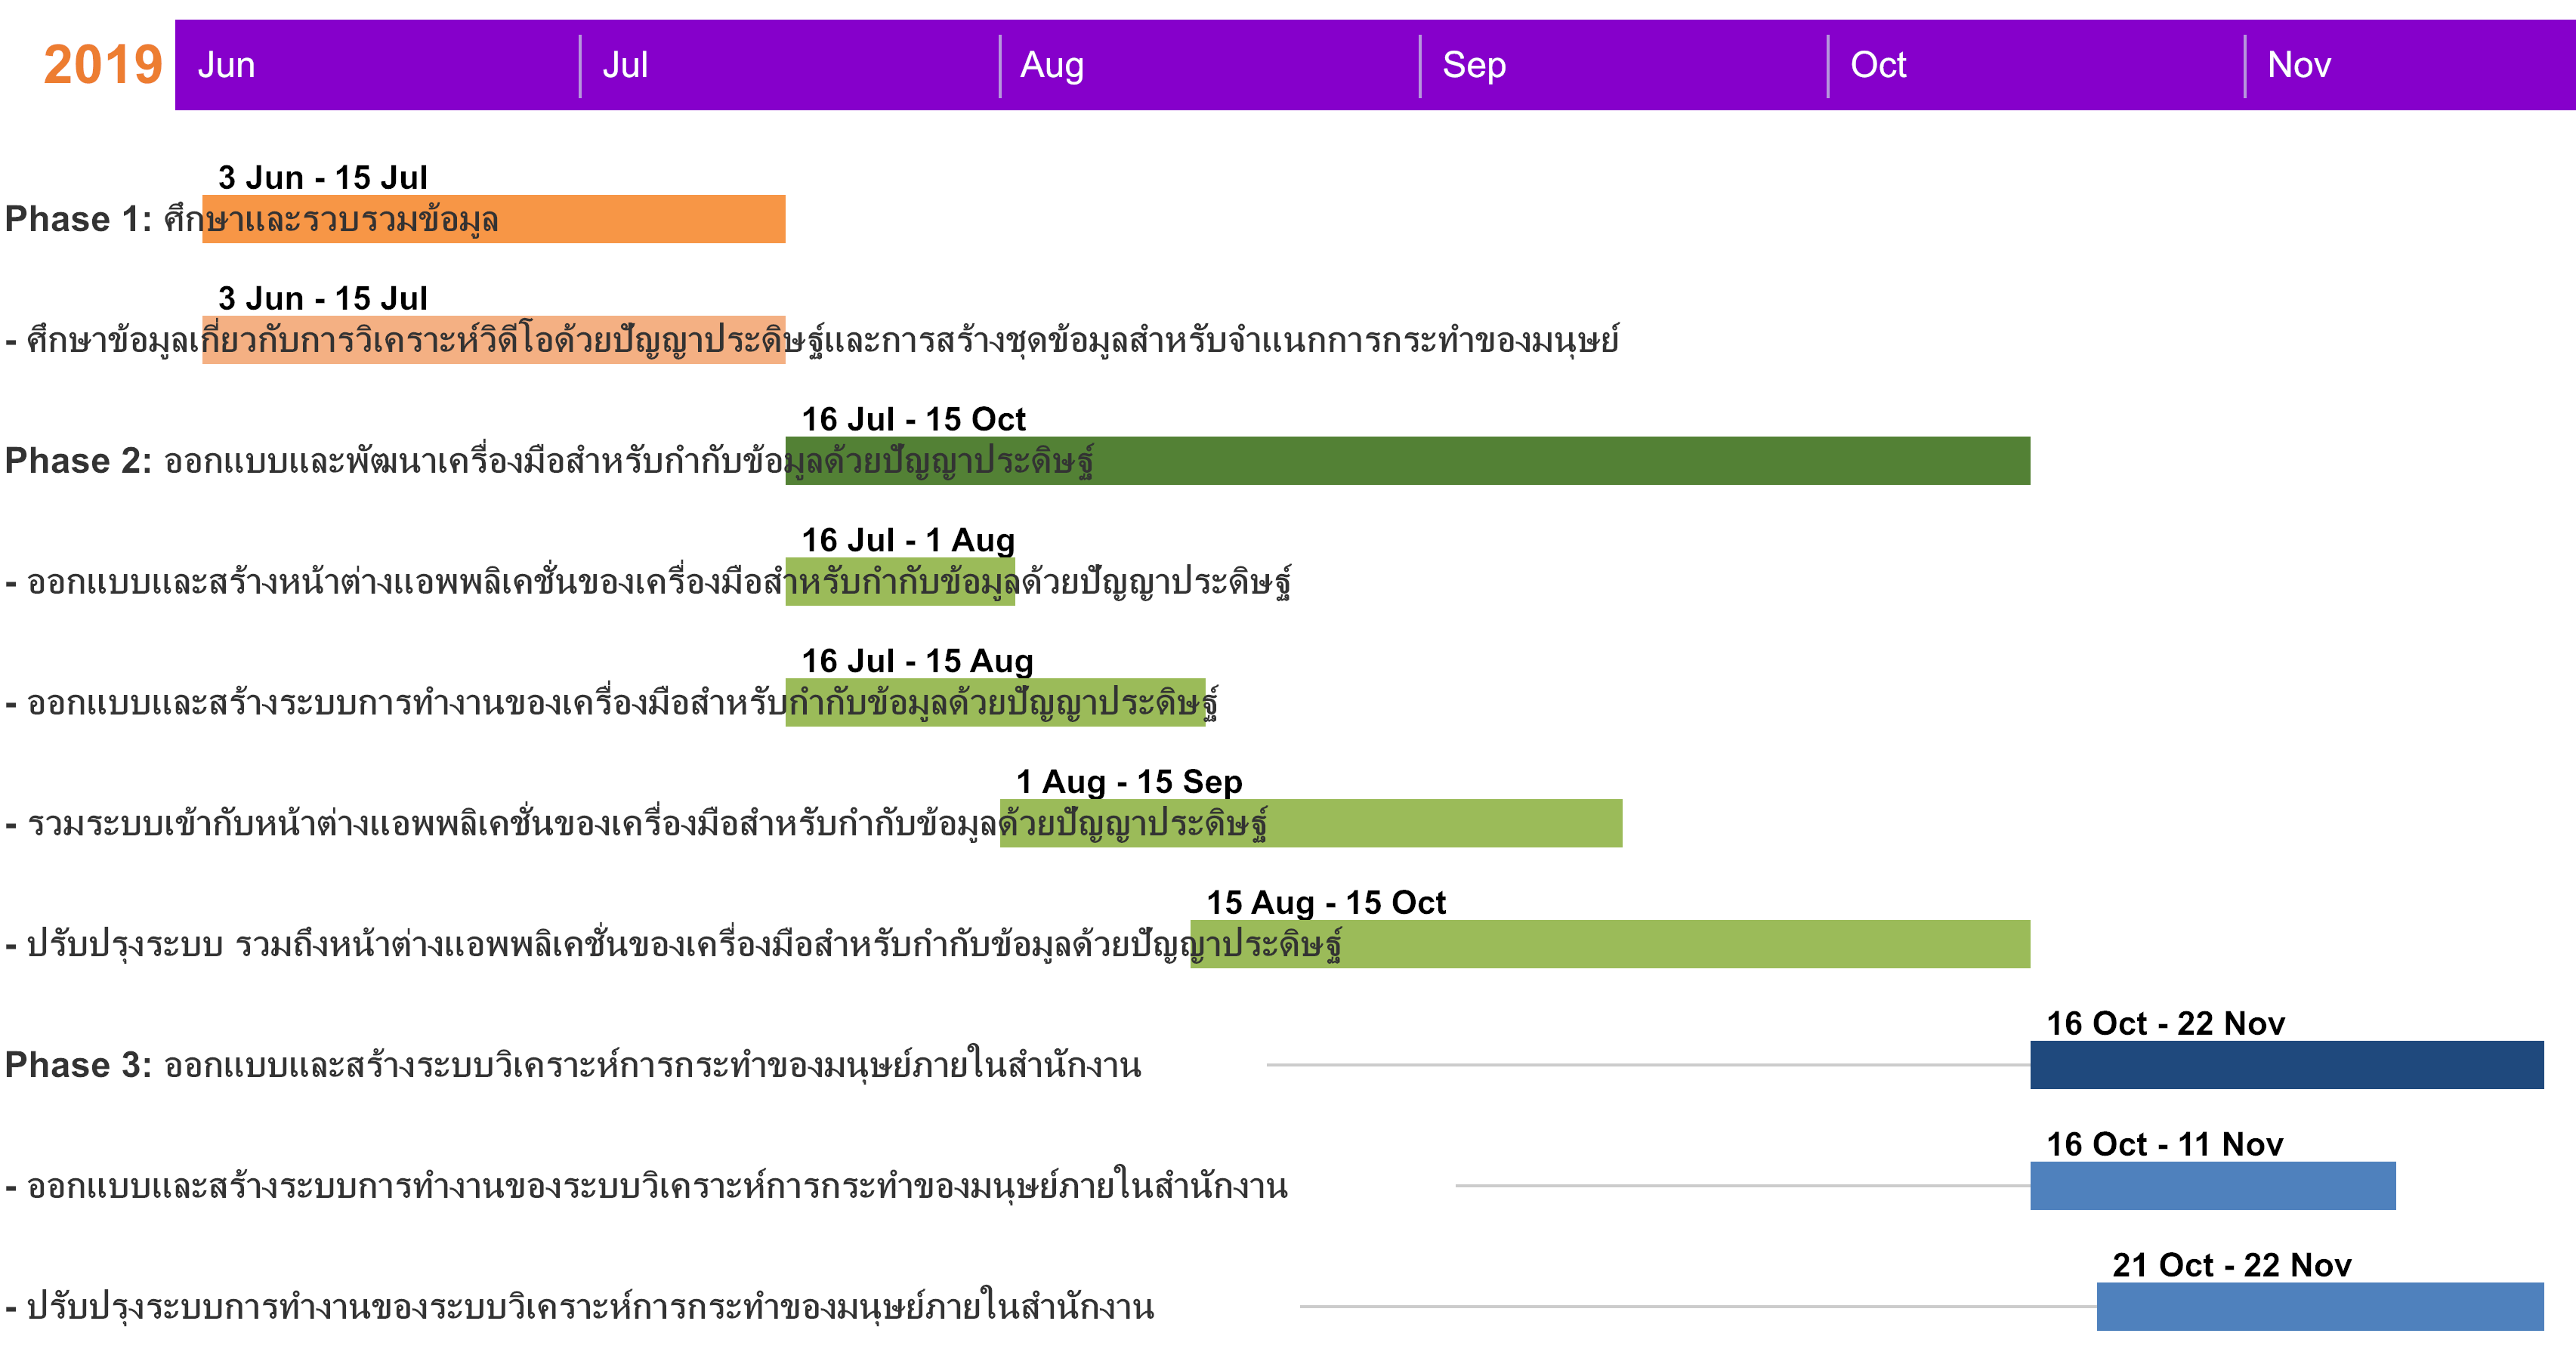
\includegraphics[width=1.125\textwidth]{chapter1/ganttchart.png}
	\caption{แผนการดำเนินงาน}
	\label{tab:ganttchart}
\end{table}
\clearpage